%!TEX root = ../dissertation.tex
\begin{savequote}[75mm]
Nulla facilisi. In vel sem. Morbi id urna in diam dignissim feugiat. Proin molestie tortor eu velit. Aliquam erat volutpat. Nullam ultrices, diam tempus vulputate egestas, eros pede varius leo.
\qauthor{Quoteauthor Lastname}
\end{savequote}

\chapter{Algorithms for Influencing Agents}
\label{ch:influencing}
There are two important components to influencing agent design: placement and
behavior.
Placement refers to the initial placement of influencing agents in the grid.
There has been some prior work on the question of how to navigate the
influencing agents to get to their initial positions
\cite{genter2015placement}, but in this work we simply place the influencing
agents in their initial positions immediately.
Behavior, on the other hand, refers to how the influencing agent changes its
orientation over time to meet its end goals.

In this chapter, we discuss placement strategies and hand-designed behaviors,
as well as our strategy for evolving new behaviors.

%Influencing agent orientation is determined by local and global behaviors.
%Local behaviors take an immediate goal direction $\theta$ and information about
%neighboring Reynolds-Vicsek agents and calculate the orientation an influencing
%agent should face to optimally direct its neighbors towards the current goal
%direction.
%Global behaviors, on the other hand, dictate how $\theta$ changes over time to
%match some final end goal.
%In some cases, this end goal may be to trace a circle around the origin; in
%this case, $\theta$ changes by a small amount every step to make sure that the
%influencing agent flies in a circle.
%In other cases, the end goal may simply be to face some final goal direction
%$\theta^*$, in which case we might have global behaviors that set
%$\theta=\theta^*$ at all times, or might change $\theta$ in some more subtle
%way.
%In this chapter, we discuss the various placement strategies and global and
%local behaviors that we study in this work.

\section{Placement Strategies}
In this work, we study a number of different placement strategies, shown in
Figure $\ref{fig:placements}$.
Except for slight modifications to make some of these strategies circular, all
the strategies are drawn from the literature \cite{genter2015placement,
genterthesis}.
\begin{figure}
    \centering
    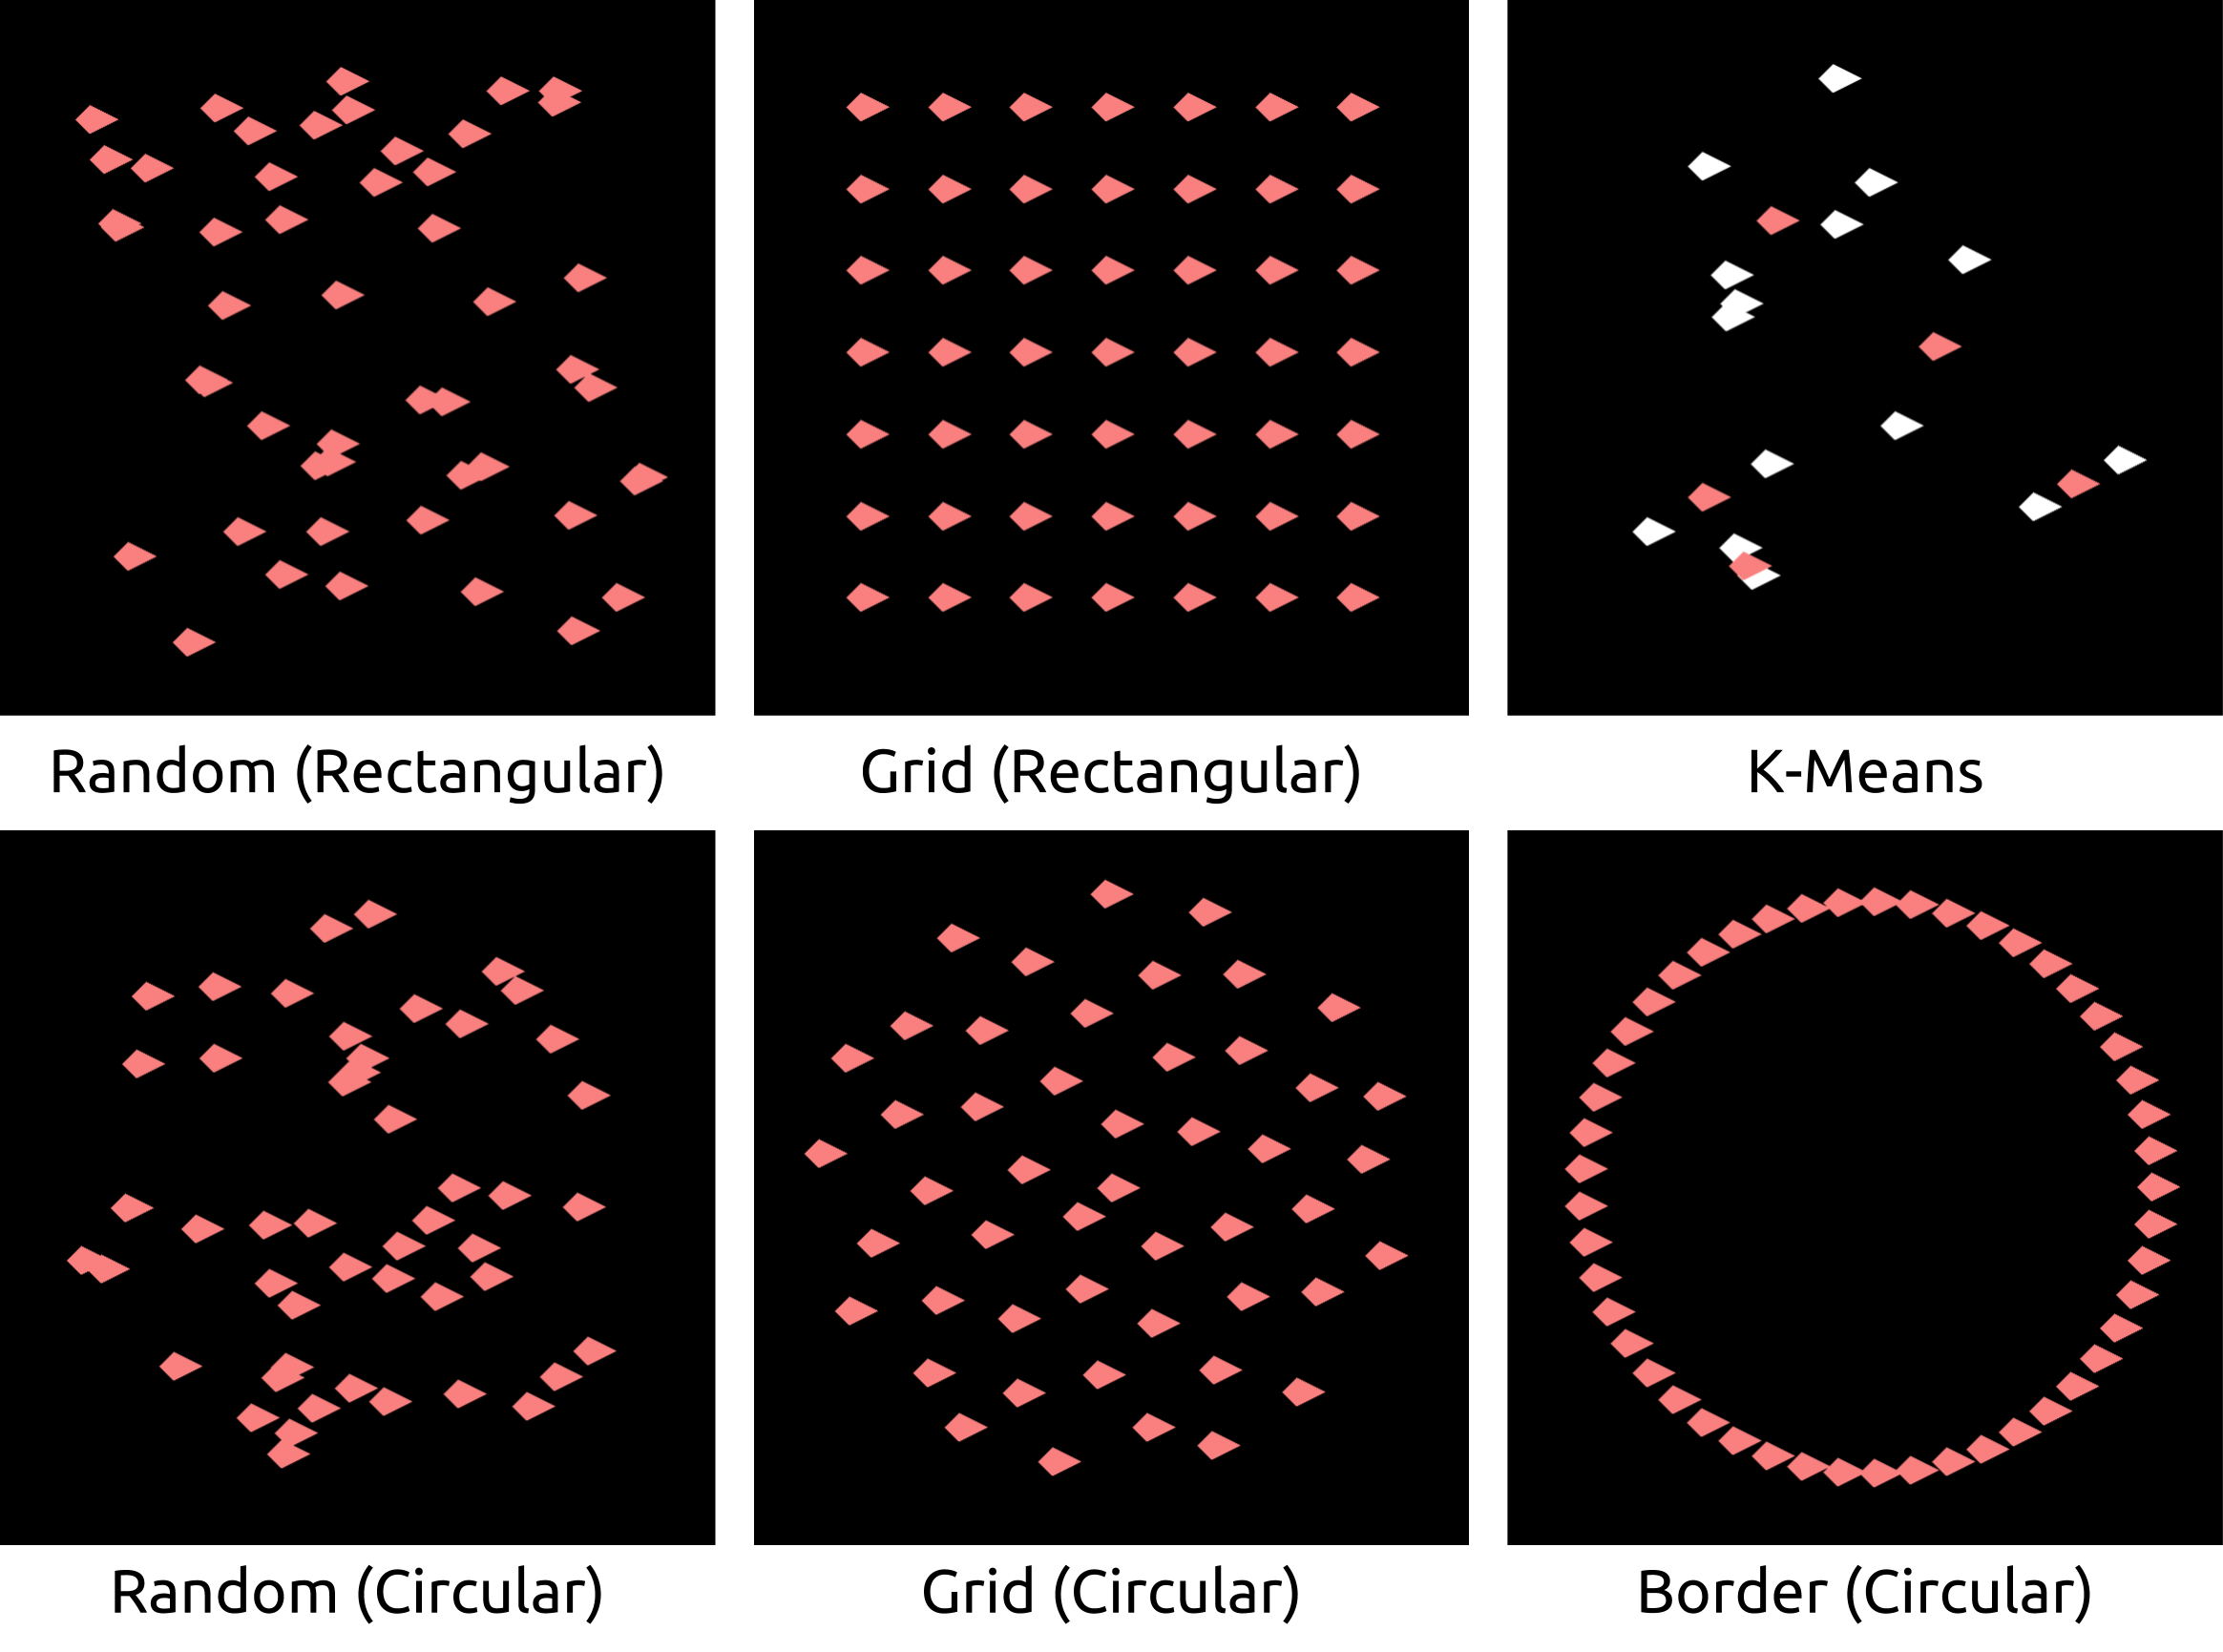
\includegraphics[width=\textwidth]{placements}
    \caption{The different placement strategies we explore in this paper.
    Red agents are influencing agents, and white agents are Reynolds-Viscek
    agents.
    Note that k-means is the only placement strategy where the placement of
    influencing agents depends on placement of Reynolds-Viscek agents.}
    \label{fig:placements}
\end{figure}
We note that the question of how to maneuver influencing agents to reach the
positions given by these placement strategies is important, but out of scope
for this paper.
For a discussion of this question, we refer the reader to Genter and Stone
\cite{genter2016facegoalfacecurrent, genterthesis}.

We use three placement strategies for the \textit{large} setting:
\textit{random}, \textit{grid}, and \textit{k-means}.
The random placement strategy, as its name suggests, places influencing agents
randomly throughout the grid.
The grid placement strategy computes a square lattice on the grid and places
influencing agents on the lattice points.
This strategy ensures regular placement of influencing agents throughout the
grid.
The k-means placement strategy uses a k-means clustering algorithm on the
positions of Reynolds-Viscek agents in the simulation space.
This strategy finds a cluster for each influencing agent by setting $k$ equal
to the number of influencing agents, and then places an influencing agent at
the center of each cluster.

We develop similar placement strategies for our \textit{herd} setting, with
some slight modifications.
To adapt the strategies to a circular arrangement of agents, we define each
strategy in terms of some radius $r$ about an origin $O$, except for the
\textit{k-means} strategy, which remains the same.
We modify the \textit{random} placement strategy to randomly distribute agents
within the circle of radius $r$ about the origin $O$, instead of the entire
simulation space.
We adapt the grid placement strategy to a circular setting using a sunflower
spiral \cite{segermansunflower}.
In polar coordinates relative to $O$, the position of the $n$-th influencing
agent in a sunflower spiral is given by $(c\sqrt{n}, \frac{2\pi}{\phi^2}n)$,
where $\phi$ is the golden ratio, and $c$ is a normalizing constant such that
the last influencing agent has distance $r$ from $O$.
We also introduce a circle border placement strategy, inspired from the border
strategies from \cite{genter2015placement}.
This strategy places agents on the circumference of the circle of radius $r$
around the origin $O$.
We refer to the circular strategies as \textit{circle-random},
\textit{circle-grid}, and \textit{circle-border}, respectively.

\section{Behaviors}
Once we have placed our influencing agents, we still need to design how they
will work together to influence the flock.
We call this aspect of the design influencing agent behaviors.
In the present work we focus on decentralized ``ad-hoc" algorithms for our
influencing agents, since this class of algorithms has been the focus of the
existing multiagent systems literature on this topic
\cite{genterthesis, genter2014neighborsorientherd, genter201612steplookahead}.
A summary of the behaviors we investigate is shown in Table
\ref{table:behaviors}.

\begin{table}[]
\footnotesize
\centering
\caption{Summary of the hand-designed behaviors we investigate}
\label{table:behaviors}
\begin{tabular}{|l|l|l|l|}
\hline
\textbf{Setting}       & \textbf{Type}               & \textbf{Name}        & \textbf{Description}                    \\ \hline
\multirow{6}{*}{Large} & \multirow{3}{*}{\textbf{}}  & \textit{Face}      & Face goal        \\ \cline{3-4}
                       &                             & \textit{Offset Momentum}      & Offset average velocity      \\ \cline{3-4}
                       &                             & \textit{One Step Lookahead}  & Simulate one step      \\ \cline{3-4}
                       &                             & \textit{Coordinated}      & Pair off and coordinate      \\ \cline{3-4}
                       &                             & \textit{Couzin}      & Averaging       \\ \cline{3-4}
                       &                             & \textit{Multistep}   & \textit{\textbf{Follow-then-influence}} \\ \hline
        \multirow{8}{*}{Herd}  & \multirow{5}{*}{Net} & \textit{Face}      & Face goal        \\ \cline{3-4}
                       &                             & \textit{Offset Momentum}      & Offset average velocity      \\ \cline{3-4}
                       &                             & \textit{One Step Lookahead}  & Simulate one step      \\ \cline{3-4}
                       &                             & \textit{Coordinated}      & Pair off and coordinate      \\ \cline{3-4}
                       &                             & \textit{Couzin}      & Averaging       \\ \cline{2-4}
                       & \multirow{3}{*}{Stationary} & \textit{Circle}      & Trace circle around agents              \\ \cline{3-4}
                       &                             & \textit{Polygon}     & Trace polygon around agents             \\ \cline{3-4}
                       &                             & \textit{Multicircle} & \textit{\textbf{Follow-then-influence}} \\ \hline
\end{tabular}
\end{table}

\subsection{Large Setting}

For the \textit{large} setting, we study four behaviors drawn from Genter and
Stone \cite{genter201612steplookahead,genter2016facegoalfacecurrent,
genter2015placement}, one behavior adapted from Couzin et. al.
\cite{couzin2005}, and one new \textit{multistep} behavior.

In previous work, Genter and Stone have introduced baseline behaviors
\textit{face} and \textit{offset momentum}, as well as more sophisticated
behaviors \textit{one step lookahead} and \textit{coordinated}.
Each of these behaviors aims to turn Reynolds-Vicsek agents to a pre-set goal
angle $\theta^*$.
In \textit{face}, influencing agents always face the angle $\theta^*$.
In \textit{offset momentum}, influencing agents calculate the average velocity
vector of the agents in their neighborhood, and take on a velocity vector that,
when added to the average velocity vector, sums to the vector pointing in
direction $\theta^*$.
In \textit{one step lookahead}, each influencing agent cycles through different
angles and simulates one step of each of its neighbors if it were to move in
that angle.
It adopts the angle that results in the smallest average difference in angle
from $\theta^*$ among all its neighbors.
Finally, in \textit{coordinated}, each agent pairs with another and runs a one
step lookahead to minimize the average difference in angle from $\theta^*$
among both their neighbors.
For a more detailed explanation of these behaviors, especially the
\textit{coordinated} behavior, we direct the reader to Genter and Stone
\cite{genter201612steplookahead}.

Couzin et. al. TALK ABOUT THE COUZIN BEHAVIOR HERE

Finally, the \textit{multistep} behavior is a novel contribution and adopts
what we call a ``follow-then-influence" behavior.
In the initial stage, influencing agents simply behave like normal Reynolds-Viscek 
agents; as a result, they easily join flocks and become distributed throughout
the grid.
At the same time, each influencing agent estimates how many Reynolds-Viscek agents
are path-connected to it; here, we define two agents as being path-connected if
there is a path between them, where edges are created by two agents being in
each other's neighborhood.
The astute reader will note that an accurate calculation requires a global view
from every influencing agent, since paths may extend arbitrarily far away from
the influencing agent.
In our algorithm, we only consider Reynolds-Viscek agents that are within the
sensing radius of the influencing agents.
Given their local estimates, the influencing agents compute a global sum of all
their estimates; once that sum passes over some threshold $T$, the influencing
agents calculate the average angle $\overline{\theta}$ among all the agents that
are locally connected to influencing agents, and from there adopt the
\textit{face} behavior with goal direction $\overline{\theta}$.
We choose $\overline{\theta}$ to minimize the amount that each influencing 
agent needs to turn its flock on average.

We also explore some variations on the \textit{multistep} behavior; notice that
once the sum of connected agents passes the threshold $T$, any of the other
behaviors studied can be used to turn the Reynolds-Vicsek agents towards the
final goal direction $\overline{\theta}$.
In other words, the \textit{multistep} behavior can be paired with any other
behavior.
We study these pairings to see how effective they are.

\subsection{Herd Setting}
For the \textit{herd} setting, we divide our behaviors into two categories:
\textit{net} behaviors and \textit{stationary} behaviors.
As a reminder, in the \textit{herd} setting, the simulation space is
non-toroidal, and all the Reynolds-Viscek agents start in a circle in the
center.
In this setting, flock formation is not guaranteed, so we are interested in
using influencing agents to instigate flocking behavior.
There are two different choices we can make; we can either try to force the
Reynolds-Viscek agents to stay in the center (\textit{stationary} behaviors),
or we can let the influencing agents direct the Reynolds-Viscek agents away
from their initial starting position (\textit{net} behaviors).
Since all our agents have a constant speed, the former is much more difficult
than the latter, so we must evaluate them separately.

For our \textit{net} behaviors, we can use all the behaviors used in the
\textit{large} setting, except for the \textit{multistep} behavior.
Since the world is non-toroidal, it is not guaranteed that the number of
connected agents will ever pass the threshold $T$; in this case, the
influencing agents would simply wander forever.

We study three \textit{stationary} behaviors: \textit{circle}, \textit{polygon},
and \textit{multicircle}.
The \textit{circle} and \textit{polygon} behaviors have each influencing agent
trace a circle or polygon around the origin.
For placement strategies where influencing agents have different distances to
the origin, the influencing agents simply trace circles and polygons of
different radii.

The \textit{multicircle} behavior is analogous to the \textit{multistep}
behavior from \textit{large}.
The influencing agents start out by circling around the origin and wait for
Reynolds-Viscek agents to enter their neighborhood.
Once they detect Reynolds-Viscek agents in their neighborhood, they adopt a
``following" behavior where they act like Reynolds-Viscek agents to integrate
into a small flock.
They continue this following stage until reaching a final radius $r_F$, at which
point they again adopt a circling behavior.
In addition to building influence by following before influencing, this behavior
also makes maintaining influence easier; since the final radius is larger than
the original radius, the final path turns less sharply than if the influencing
agents had stayed at their original radius.
To the best of our knowledge, this is the first presentation of such a
multi-stage behavior to induce circling behavior under the Reynolds-Vicsek
model in the literature.

%To help organize our analysis, we split behaviors into local and global
%components; each influencing agent behavior is composed of a local and global
%component.
%The local component takes a desired orientation as an argument and dictates
%which direction an influencing agent will face to try to influence its neighbors
%towards the goal orientation.
%The global component, on the other hand, dictates the desired orientation to
%feed to the local component and how the influencing agents might coordinate to
%decide on a desired orientation.
%For example, one behavior might be for the influencing agents to circle around
%the center of a grid and get the Reynolds-Viscek agents to circle with them.
%The global component would compute the desired orientation necessary at each
%step to maintain the circling behavior, and the local component would compute
%which exact direction to face to get the Reynolds-Viscek agents to face the
%desired orientation at that step.
%For grammatical sanity, we will refer to different candidates for local and
%global components as ``local behaviors" and ``global behaviors" throughout the
%rest of this paper; however, it is important to recognize that any actual
%behavior must have a local and global component.
%
%\subsection{Local Behaviors}
%Like our placement strategies, we draw on Genter and Stone for many of our
%local behaviors \cite{genter201612steplookahead,genter2016facegoalfacecurrent,
%genter2015placement}.
%In previous work, they have introduced baseline behaviors \textit{face} and
%\textit{offset momentum}, as well as more sophisticated behaviors \textit{one
%step lookahead} and \textit{coordinated}.
%Each of these behaviors requires a goal angle $\theta^*$.
%In \textit{face}, influencing agents always face the angle $\theta^*$.
%In \textit{offset momentum}, influencing agents calculate the average velocity
%vector of the agents in their neighborhood, and take on a velocity vector that,
%when added to the average velocity vector, sums to the vector pointing in
%direction $\theta^*$.
%In \textit{one step lookahead}, each influencing agent cycles through different
%angles and simulates one step of each of its neighbors if it were to move in
%that angle.
%It adopts the angle that results in the smallest average difference in angle
%from $\theta^*$ among all its neighbors.
%Finally, in \textit{coordinated}, each agent pairs with another and runs a one
%step lookahead to minimize the average difference in angle from $\theta^*$
%among both their neighbors.
%For a more detailed explanation of these behaviors, especially the
%\textit{coordinated} behavior, we direct the reader to Genter and Stone
%\cite{genter201612steplookahead}.
%
%\subsection{Global Behaviors}
%TODO: ADD COUZIN VERSION, ADD OTHER NET BEHAVIORS, ADD BEHAVIORS THAT DIDN'T
%MAKE IT?
%
%The global behaviors we investigate are listed in Table \ref{table:global}.
%Again, we use the same global behaviors for the \textit{large} and
%\textit{small} settings: \textit{direct}, \textit{random}, and
%\textit{multistep}.
%As its name suggests, the \textit{direct} global behavior has each influencing
%agent use a local behavior to directly influence its neighbors towards the
%goal angle $\theta^*$.
%When an influencing agent has no neighbors, it simply faces the goal direction.
%
%\begin{table}[]
%\footnotesize
%\centering
%\caption{Summary of global behaviors we investigate}
%\label{table:global}
%\begin{tabular}{|l|l|l|l|}
%\hline
%\textbf{Setting}       & \textbf{Type}               & \textbf{Name}        & \textbf{Description}                    \\ \hline
%\multirow{3}{*}{Large} & \multirow{3}{*}{\textbf{}}  & \textit{Direct}      & Influence neighbors or face goal        \\ \cline{3-4}
%                       &                             & \textit{Random}      & Influence neighbors or face random      \\ \cline{3-4}
%                       &                             & \textit{Multistep}   & \textit{\textbf{Follow-then-influence}} \\ \hline
%\multirow{4}{*}{Herd}  & Net                         & \textit{Direct}      & Influence neighbors or face goal        \\ \cline{2-4}
%                       & \multirow{3}{*}{Stationary} & \textit{Circle}      & Trace circle around agents              \\ \cline{3-4}
%                       &                             & \textit{Polygon}     & Trace polygon around agents             \\ \cline{3-4}
%                       &                             & \textit{Multicircle} & \textit{\textbf{Follow-then-influence}} \\ \hline
%\end{tabular}
%\end{table}
%
%The \textit{random} global behavior is very similar, but it directs influencing
%agents in a random direction when they have no Reynolds-Viscek neighbors.
%We introduced this behavior as a response to interactions where an influencing
%agent is almost successful in changing the direction of a group of Reynolds-Viscek
%agents, but gets separated before it is completely successful.
%In these cases, the Reynolds-Viscek agents are left on a trajectory that is almost
%parallel to the goal direction; as a result, further interactions with
%influencing agents are rare.
%
%The \textit{multistep} behavior is a novel contribution and adopts what we call
%a ``follow-then-influence" behavior.
%In the initial stage, influencing agents simply behave like normal Reynolds-Viscek 
%agents; as a result, they easily join flocks and become distributed throughout
%the grid.
%At the same time, each influencing agent estimates how many Reynolds-Viscek agents
%are path-connected to it; here, we define two agents as being path-connected if
%there is a path between them, where edges are created by two agents being in
%each other's neighborhood.
%The astute reader will note that an accurate calculation requires a global view
%from every influencing agent, since paths may extend arbitrarily far away from
%the influencing agent.
%In our algorithm, we only consider Reynolds-Viscek agents that are within the
%sensing radius of the influencing agents.
%Given their local estimates, the influencing agents compute a global sum of all
%their estimates; once that sum passes over some threshold $T$, the influencing
%agents calculate the average angle $\overline{\theta}$ among all the agents that
%are locally connected to influencing agents, and from there adopt the
%\textit{direct} behavior with goal direction $\overline{\theta}$.
%We choose $\overline{\theta}$ to minimize the amount that each influencing 
%agent needs to turn its flock on average.
%
%For the \textit{herd} setting, we divide our global behaviors into two
%categories: \textit{net} behaviors and \textit{stationary} behaviors.
%As a reminder, in the \textit{herd} setting, the simulation space is
%non-toroidal, and all the Reynolds-Viscek agents start in a circle in the
%center.
%In this setting, flock formation is not guaranteed, so we are interested in
%using influencing agents to instigate flocking behavior.
%There are two different choices we can make; we can either try to force the
%Reynolds-Viscek agents to stay in the center (\textit{stationary} behaviors),
%or we can let the influencing agents direct the Reynolds-Viscek agents away
%from their initial starting position (\textit{net} behaviors).
%Since all our agents have a constant speed, the former is much more difficult
%than the latter, so we must evaluate them separately.
%
%The \textit{net} behavior is equivalent to the \textit{direct} behavior; there
%is a single pre-determined goal direction, and the influencing agents try to
%direct the Reynolds-Viscek agents towards the goal direction.
%We call it a net behavior because it looks as if the influencing agents are
%``catching" the Reynolds-Viscek agents in a net.
%
%We study three \textit{stationary} behaviors: \textit{circle}, \textit{polygon},
%and \textit{multicircle}.
%The \textit{circle} and \textit{polygon} behaviors have each influencing agent
%trace a circle or polygon around the origin.
%For placement strategies where influencing agents have different distances to
%the origin, the influencing agents simply trace circles and polygons of
%different radii.
%
%The \textit{multicircle} behavior is analogous to the \textit{multistep} behavior
%from \textit{large}.
%The influencing agents start out by circling around the origin and wait for
%Reynolds-Viscek agents to enter their neighborhood.
%Once they detect Reynolds-Viscek agents in their neighborhood, they adopt a
%``following" behavior where they act like Reynolds-Viscek agents to integrate
%into a small flock.
%They continue this following stage until reaching a final radius $r_F$, at which
%point they again adopt a circling behavior.
%In addition to building influence by following before influencing, this behavior
%also makes maintaining influence easier; since the final radius is larger than
%the original radius, the final path turns less sharply than if the influencing
%agents had stayed at their original radius.
%To the best of our knowledge, this is the first presentation of such a
%multi-stage behavior to induce circling behavior under the Reynolds-Vicsek model in
%the literature.
%
%Besides the above global behaviors, we also explored a few more variations on
%the \textit{net} behavior and the \textit{multicircle} behavior.
%One variation of the \textit{net} behavior was equivalent to the \textit{random}
%global behavior from the large setting.
%The other was similar to the stationary \textit{circle} behavior; influencing
%agents would trace a circle until encountering Reynolds-Viscek agents,
%whereupon they would influence the Reynolds-Viscek agents towards the goal
%direction.
%The variations on the \textit{multicircle} behavior included different final
%radii from those presented in $\S\ref{sec:evaluation}$, as well as a variation
%that introduced a transitional period between the initial following state and
%the final circling state.
%These additional variants added few qualitative insights, so we do not report
%them for simplicity of exposition.

% This behavior is parameterized by three variables, a placement radius $r_P$, a
% threshold radius $r_T$ and a final radius $r_F$.
% A diagram of this behavior is shown in $\ref{fig:multicircle}$.
% \begin{figure}
%     \centering
%     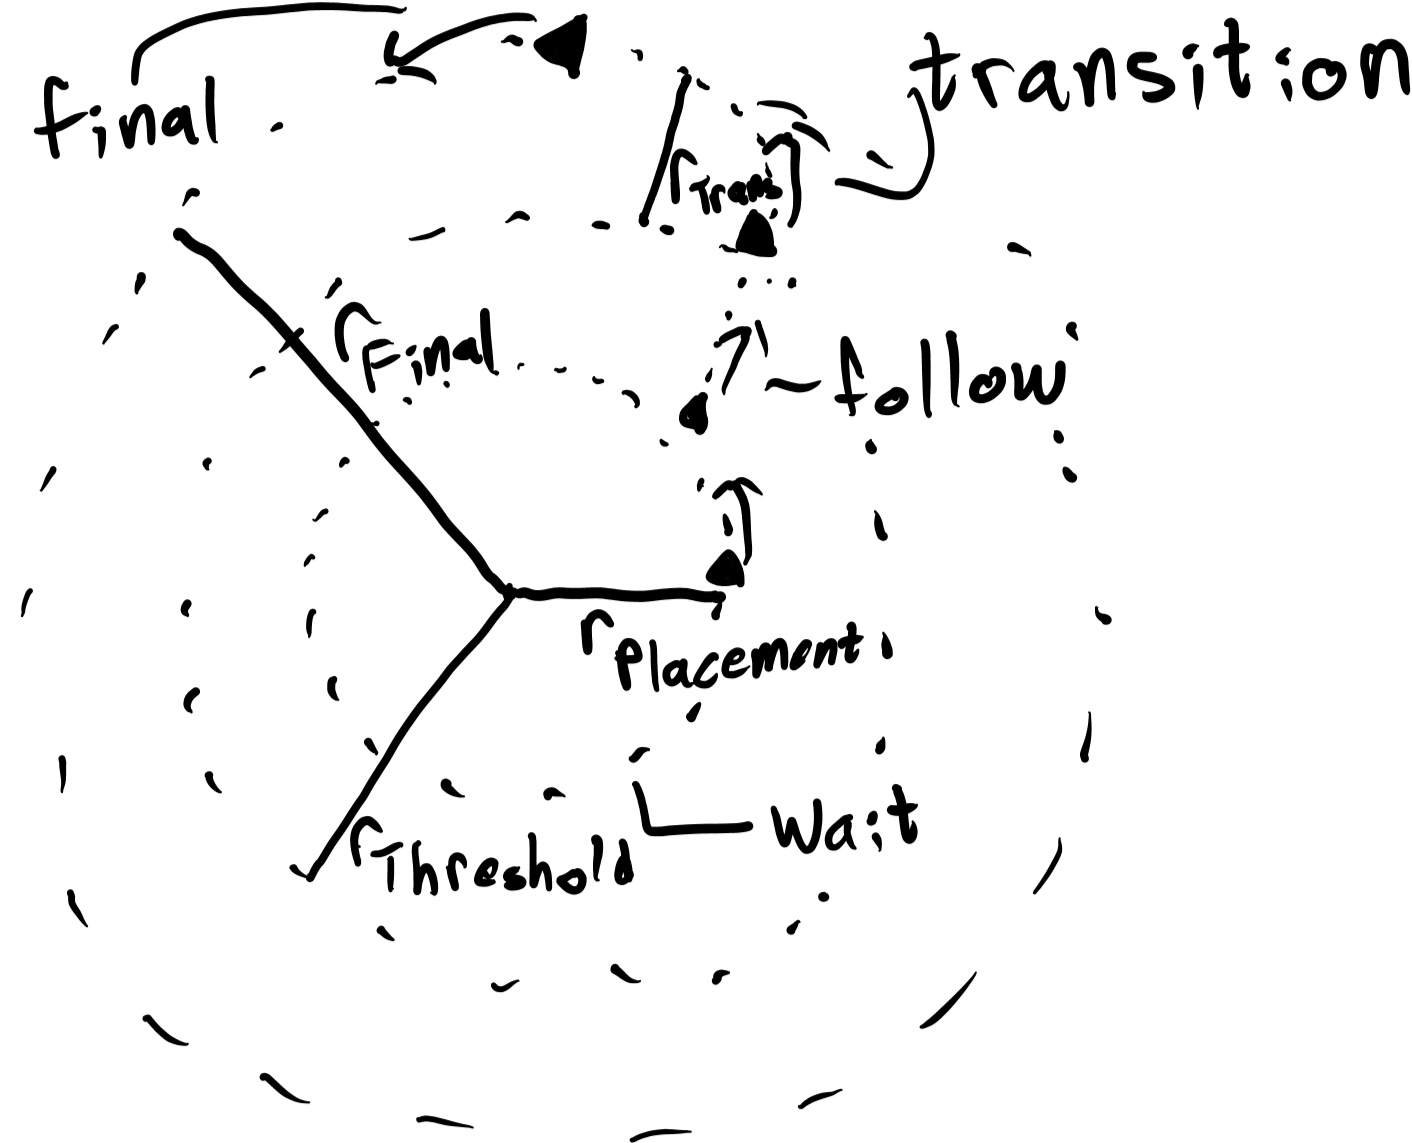
\includegraphics[width=0.5\textwidth]{multicircle}
%     \caption{A diagram of the \textit{multicircle} global behavior. NOTE: WE WILL REPLACE THIS WITH A NON-SKETCH}
%     \label{fig:multicircle}
% \end{figure}
% Agents start by tracing a circle around the origin of radius $r_P$; $r_P$ is
% defined by the agent's placement under the placement strategy.
% Once the agents come into contact with Reynolds-Viscek agents, they follow the Reynolds-Viscek
% agents until they reach a threshold radius $r_T$.
% From there, they trace a transition path until they are a radius $r_F$ from the
% origin, where they settle into a final trajectory tracing the circle of radius
% $r_F$ around the origin.

% We compute the transition path by finding a circle that is tangent to both the
% influencing agent's velocity vector when it is at radius $r_T$ and the final
% circle of radius $r_F$.
% This problem reduces to one of geometry; we wish to find a point $O'$ around
% which to trace a transition circle.
% For the rest of this computation, assume that the influencing agent is at the
% threshold radius $r_T$.

% We can reduce the set of candidate points by taking the line orthogonal to the
% agent's velocity vector that intersects the agent's velocity vector at the
% agent's position.
% Consider a point $O'$ on this line, and let $r'$ be the distance of
% $O'$ from the agent.
% Then, the circle of radius $r'$ centered around $O'$ is tangent to
% the agent's velocity vector at the agent's position.
% Since we know the form of the line that $O'$ is on, we simply need to
% determine a proper radius $r'$.

% We have one more condition: that the transition circle be tangent to the larger
% circle.
% For this to be the case, we must have that the distance from $O'$ to the
% larger circle be $r'$.
% Let $r_{O}$ be the distance from $O'$ to the origin of the larger circle.
% Then we have $r' = r_F - r_{O}$.
% This gives us the proper value of $r'$, and two candidates for $O'$.
% We choose the point that causes the agent to enter the larger circle clockwise,
% to prevent collisions on the larger circle.
% During the actual simulations, we calculate this point numerically, walking
% along both sides of the orthogonal line until finding the right candidate.

\section{Evolving Behaviors}
To evolve behaviors, we run genetic algorithms over genomes containing
abstract syntax trees for a simple domain specific language we designed
specifically for computing a new heading from a list of neighboring agents.

\subsection{Domain Specific Language}
All evolved behaviors need to be well-defined for any number of
neighboring agents, so we choose an execution model that generalizes over the
number of neighbors a influencing agent has.
Every expression in our domain specific language defines a function from an
accumulator value representing a heading and a neighbor agent to a new
accumulator value.
Starting with an initial accumulator value, the same function is applied to
each of the influencing agent's neighbors in decreasing order of distance.
The result of each application becomes the accumulator value fed to the next
application, and the result of the final application is the heading the
influencing agent will take in the next time step.
In functional programming terms, we are evolving a function used to fold over a
list of neighbors.
The pseudocode for this fold is in listing \ref{listing:fold}.

\begin{lstlisting}[caption={A fold},captionpos=b,label={listing:fold}]
acc = initial_acc
for neighbor in neighbors:
    acc = f(acc, neighbor)
return acc
\end{lstlisting}

The order in which neighbors are evaluated is meaningful, since the evolved
functions are not necessarily commutative.
We choose to evaluate them in decreasing order of distance to ensure that the
results of programs that do not use the accumulator value are determined by the
nearest neighbor of the influencing agent.
If the influencing agent has no neighbors, its calculated heading is equal to
its initial accumulator value.
A genome is comprised of an abstract syntax tree for the folding function and
the initial accumulator value.
The initial accumulator value is either the influencing agent's current heading
or the goal direction, decided at random when an initial genome is created.
An example of a hand-crafted genome is given in listing
\ref{listing:example_genome}.

\begin{lstlisting}[caption={A small genome that sets the agent's heading to the
average of its neighbors' headings},captionpos=b,label={listing:example_genome}]
acc=current;
(add acc (mul influence heading))
\end{lstlisting}

By using a fold as our execution model, we can keep the syntax of the language
very simple.
Because the execution model handles looping over the list of neighbors, there
is no need for the language itself to have syntax expressing loops or lists.
Although allowing the language to have lists and loops would increase its
expressiveness, we opted to keep the language simple while still expressive
enough to allow the genetic algorithm to develop complex behaviors.
We also chose to leave out other possible capabilities such as mechanisms for
storing state other than the accumulator value and communicating with other
influencing agents.

The expressions that make up the domain specific language are given in table
\ref{table:lang_exprs}.
When evaluated, every expression in the language has a value in the range
$[-1,1]$, which is interpreted as an angle (in radians) by multiplying by
$\pi$.
All angles are relative to the influencing agent's current heading.
Addition, subtraction, sine, and cosine operators treat their arguments as
angles, but multiplication, exponentiation, arcsine, and arccosine treat them
as scalar values.
Division is purposefully excluded from the language because there is no
meaningful way to enforce that its result is in the range $[-1, 1]$.
Exponentiation is modified such that the exponent is implicitly shifted into
the range $[0, 2]$ to enforce the same invariant.

We determined what information should be made available about neighboring
agents by drawing on our own intuition about what information would be valuable
in designing an influencing behavior, then transforming it to be in the range
$[-1, 1]$.
For example, knowing the index of the current neighbor allows for creating a
function that gives more weight to closer neighbors (those with higher indices);
knowing the distance to the current neighbor combined with the conditional
expression, gez, allows for creating programs that ignore neighbors that are
too close or too far away;
and the product of the influence variable and some other value can be added to
the accumulator to calculate an average over all neighbors.
Figure \ref{fig:genome_diagram} shows how the direction, distance, heading, and
goal variables relate to the position of a neighboring agent.

\begin{table}[h]
\centering
\begin{tabular}{|c|c|} 
    \hline
    \textbf{Expression} & \textbf{Semantics} \\
    \hline
    direction & angle toward neighbor\\ \hline
    distance & distance to neighbor / sensing radius \\ \hline
    heading & relative heading of neighbor \\ \hline
    influence & 1 / \# of neighbors \\ \hline
    index & index of neighbor / \# of neighbors\\ \hline
    goal & angle toward goal direction \\ \hline
    acc & the accumulator value \\ \hline
    $f$ & some constant $f \in [-1, 1]$ \\ \hline
    (sin $e$) & $\sin(e\cdot\pi)$\\ \hline
    (cos $e$) & $\cos(e\cdot\pi)$\\ \hline
    (asin $e$) & $2\cdot\text{asin}(e)/\pi$\\ \hline
    (acos $e$) & $2\cdot\text{acos}(e)/\pi - 1$\\ \hline
    (add $e_1$ $e_2$) & $\text{wrap}_{[-1,1]}(e_1 + e_2)$ \\ \hline
    (sub $e_1$ $e_2$) & $\text{wrap}_{[-1,1]}(e_1 - e_2)$\\ \hline
    (mul $e_1$ $e_2$) & $e_1 \cdot e_2$\\ \hline
    (exp $e_1$ $e_2$) & $e_1^{e_2+1}$\\ \hline
    (gez $e_1$ $e_2$ $e_3$) & if $e_1 >= 0$ then $e_2$ else $e_3$ \\ \hline
\end{tabular}
\caption{Language expressions}
\label{table:lang_exprs}
\end{table}
\begin{figure}
    \centering
    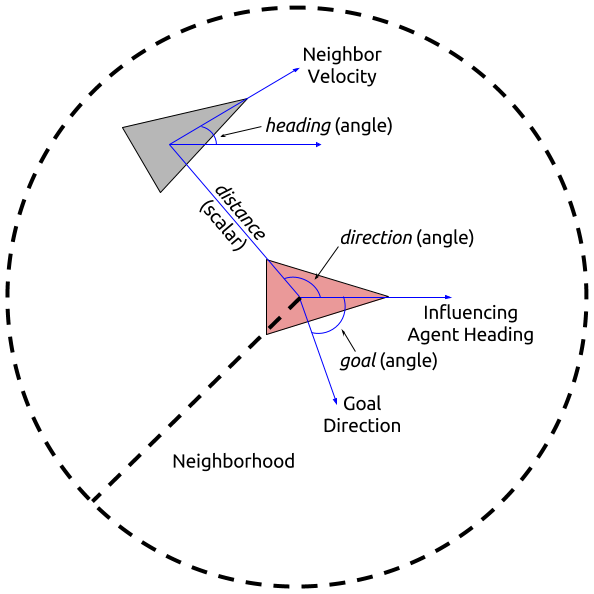
\includegraphics[width=\textwidth]{genomediagram}
    \caption{Some of the variables used in the domain-specific language.}
    \label{fig:genome_diagram}
\end{figure}

To keep the language simple, angular and scalar values are used
interchangeably.
Introducing a type system to keep them separate would greatly reduce the space
of programs the genetic algorithm has to search through, at the expense of
complicating the genetic operators, which would have to respect such a type
system.
We leave implementing such a type system as well as implementing a richer
language as future work.

\subsection{Evolutionary Algorithm}
\label{sec:evolutionaryalg}
The two genetic operators we use in our genetic algorithm are the classic
operators in genetic programming, crossover and mutation \cite{deCastro2007}.
Crossover works by picking a random subtree from each of two abstract syntax
trees and swapping them.
Mutation picks a node at random from an abstract syntax tree and changes it
into some new node, picked uniformly at random from the set of expression types
available in the language.
The children of the old node are made children of the new node in random order,
although children may be lost if the new node has fewer children than the old
node and new children may need to be randomly generated if the new node has
more than the old node.

We start by randomly generating each member of the population.
We evaluate each member with $6$ Reynolds-Viscek agents in a small test setting,
calculating the average absolute difference in angle of the Reynolds-Viscek
agents from the goal direction after $100$ steps.
This gives a positive fitness value that we wish to optimize towards zero.
In each generation, we choose the top $N$ genomes to use as a seed population
for the next generation, where $N$ is a hyperparameter set by the user.
We add those $N$ genomes into the new population.
Then, while the size of the new population is smaller than the size of the
old population, we repeat the following:
\begin{enumerate}
    \item Flip a coin to decide whether to create a new member(s) by mutation
    or crossover.
    \item If mutation, randomly select one genome from the seed population,
    mutate it, and add it to the new population.
    \item If crossover, randomly select two genomes from the seed population,
    and use them to perform crossover.
    This creates two new offspring; add them both if there is room, otherwise
    randomly select one to add.
\end{enumerate}

We experimented with a few variations on this algorithm over the course of this
work.
We started by choosing one individual in each generation to mutate, and randomly
replaced one individual, chosen proportionally to fitness (keeping in mind that
closer to $0$ is better).
However, it was difficult for this algorithm to favor better candidates, since
fitness values were so close to each other.
We tried switching to a rank-proportional replacement algorithm, but this
approach had the opposite problem of distinguishing too finely between genomes
with very similar fitness.
We ultimately settled on our seed population approach as a compromise between
these two forces.
We also initially evolved genomes without the bias towards shorter genomes,
but we found that this led to blow-out as soon as we added crossover.
